\documentclass[tikz,border=5pt]{standalone}
\definecolor{myyellow}{RGB}{224,239,158}
\definecolor{myteal}{RGB}{47,89,85}

\begin{document}
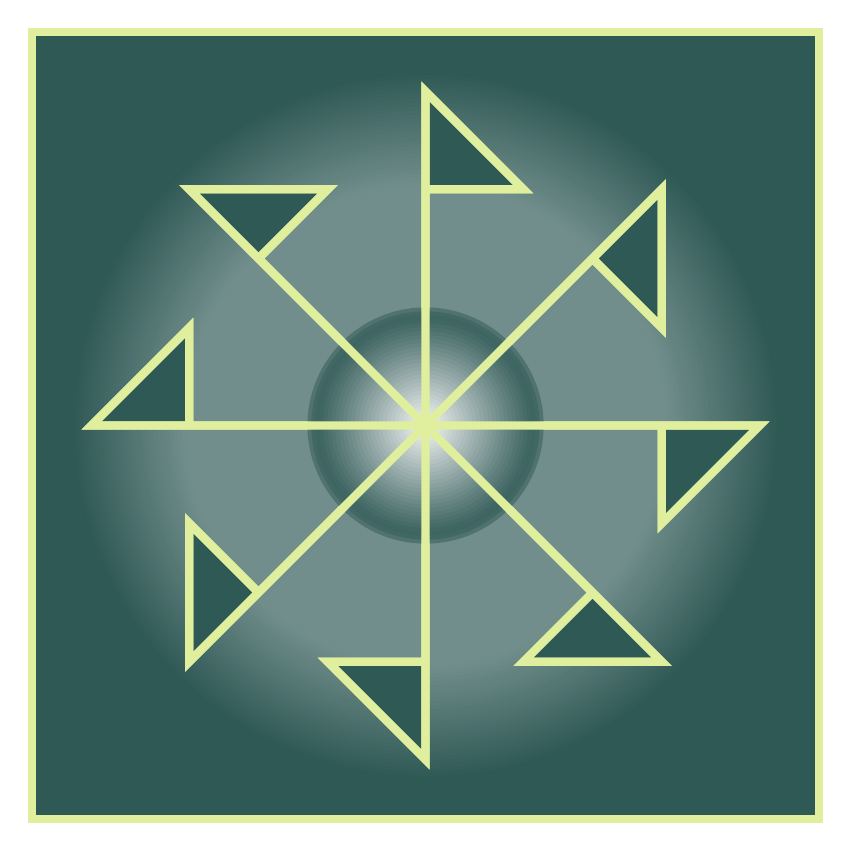
\begin{tikzpicture}[
    cover/.style={line width=3pt,myyellow},
    coverfill/.style={cover,fill=myteal},
    myrect/.pic={
        \draw[#1] (0,0) -- (3,3)
            -- ++(0,-\fpeval{3*(2-sqrt(2))})
            -- (45:3) -- cycle;
    }
]

% bottom glow
\draw[coverfill] (-5,-5) rectangle (5,5);
\foreach \i in {4.5, 4.45, ..., 3} {
    \def\tmp{\fpeval{100*(\i/4.5)}}
    \fill[myteal!\tmp!white] circle[radius=\i cm];
}

% arms filled
\foreach \i in {0,45,90,...,315} {
    \pic[rotate=\i] {myrect={coverfill}};
}

% top glow
\foreach \i in {1.5, 1.45, ..., 0} {
    \def\tmp{\fpeval{100*(\i/1.5)}}
    \fill[myteal!\tmp!white,opacity=0.5] circle[radius=\i cm];
}

% arms border
\foreach \i in {0,45,90,...,315} {
    \pic[rotate=\i] {myrect={cover}};
}

\end{tikzpicture}
\end{document}